\documentclass[10pt,onecolumn,openright]{book}

% Configure title, author, etc of the thesis in TexFiles/settings.tex

%================================================================%
%  All packages and new commands are treated in an own document  %
%================================================================%
%%=========================================================================%
%%                               Settings                                  %
%%=========================================================================%

%Comment out or remove if it's a Licentiate thesis!
%\def\phdThesis{1}

% Important commands for this thesis!
\newcommand{\currentyear}{2023}
\newcommand{\authorname}{Robert Krook}
\newcommand{\mytitle}{High-level Programming on Low-level Platforms}
\newcommand{\mysubtitle}{Two Domain-specific Languages based on Haskell} % Comment out if you don't want a subtitle

\newcommand{\division}{Computer Science and Engineering}
%\newcommand{\researchgroup}{Some Research Group} % Comment out if not applicable


%PHD ONLY
\newcommand{\phdISBN}{xxx-xx-xxxx-xxx-x}
\newcommand{\phdSeriesNumber}{xxxx}
\newcommand{\techReportNumber}{XXXX}


%==============%
% Other common strings, these might need to be changed to follow updated guidelines

\newcommand{\licISSN}{1652-876X}
\newcommand{\phdISSN}{0346-718X}

\newcommand{\chalmers}{Chalmers University of Technology}
\newcommand{\gotuni}{University of Gothenburg}
\newcommand{\mydepartment}{Department of Computer Science and Engineering}
\newcommand{\chalIgu}{\chalmers~\IfItalicsTF{$|\!$}{$|$}~\gotuni} % The \! (negative thin space) is to fix kerning because italics seems to add extra space on the right of the inline math
\newcommand{\chalandgu}{\chalmers~and~\gotuni}

\ifx\phdThesis\undefined
\newcommand{\degreetitle}{Licentiate of Engineering}
\else
\newcommand{\degreetitle}{Doctor of Philosophy}
\fi


\ifx\phdThesis\undefined
%reportNo is not used for lic anymore, but double check with the intranet.
%in case you need it just uncomment the text in the identifierNoText command.
\newcommand{\identifierNoText}{%Technical Report No \techReportNumber \\
ISSN \licISSN\\
}
\else
\newcommand{\identifierNoText}{ISBN \phdISBN\\
Doktorsavhandlingar vid Chalmers tekniska h\"{o}gskola, Ny serie nr \phdSeriesNumber .\\
ISSN \phdISSN\\
Technical Report No. \techReportNumber \\
\vspace{1.5cm}
}
\fi




%%=========================================================================%
%%                               Settings                                  %
%%=========================================================================%
\setlength{\headheight}{14mm}

% G5 format
\usepackage{geometry}

\ifx\inlagaPage\undefined
% Thesis is paper size G5
\geometry{paperwidth=169mm, paperheight=239mm, inner=28mm,outer=22mm,top=22mm, bottom=18mm}
\else
% Presentation sheet uses paper size A5
\geometry{paperwidth=148mm, paperheight=210mm, inner=25mm,outer=25mm,top=22mm, bottom=18mm}
\fi

%-----------------------Used packages---------------------------------------------------------%
\usepackage{fancyhdr}
\pagestyle{fancy}
\fancyhead[LE,RO]{\thepage}
\fancyhead[RE]{\scriptsize \slshape \leftmark}
\fancyhead[LO]{\scriptsize \slshape \rightmark}
\fancyfoot[C]{}

\setcounter{secnumdepth}{3} \setcounter{tocdepth}{3}

\usepackage[labelformat=simple]{subcaption}
\renewcommand\thesubfigure{(\alph{subfigure})}
\usepackage{graphicx}
\usepackage{url}
%\usepackage{cite}
% \usepackage{multibib}

%\usepackage[english]{babel}
\usepackage[british]{babel} % Using english will cause dates in the bibliography to be mm-dd-yyyy, instead of the more proper dd-mm-yyyy
\usepackage[backend=bibtex,style=ieee,maxcitenames=3,backref=true,language=british]{biblatex} 
%Different styles depending on whether you want numeric/alphabetic citation key
% style=ieee
% style=apa
\addbibresource{references.bib}

\usepackage{amsmath,amssymb,amscd,latexsym,dsfont}
%\usepackage[latin1]{inputenc}
%\usepackage{amsmath}
%\usepackage{amssymb}
%\usepackage{latexsym}
\usepackage{textcomp}
% \usepackage{multirow}
% \usepackage{multicol}
\usepackage{psfrag}
\usepackage{rotating}
%\usepackage{xspace}
%\usepackage{enumerate}
\usepackage{enumitem}
\usepackage{pdflscape}


\usepackage[final]{pdfpages}
\usepackage{xspace}
\usepackage{relsize}

\usepackage{url}
\usepackage{IEEEtrantools}

% \usepackage{fixltx2e}

\usepackage{microtype}

\usepackage[textsize=tiny,textwidth=20mm,backgroundcolor=orange!70]{todonotes}
\setlength{\marginparwidth}{20mm} % This is so the notes don't get cut out of the page



%----------Some commands you can use-----------%

\newcommand{\figref}[1]{Fig.~\ref{#1}}
\newcommand{\tabref}[1]{Table~\ref{#1}}
\newcommand{\chapref}[1]{Chap.~\ref{#1}}
\newcommand{\secref}[1]{Section~\ref{#1}}
\newcommand{\eqnref}[1]{Equation~\ref{#1}}
\newcommand{\paperref}[1]{Paper~\romannum{#1}}

%use this command to denote figure element that appear inside a figure
\newcommand{\fe}[1]{\textsf{\small #1}}

\newcommand{\p}[1]{\textsf{\small #1}}

\newcommand{\interviewquote}[2]{\begin{quote}
\footnotesize{\emph{``#1'' }} --- \footnotesize{#2}
\end{quote} }



%----------Some commands we need-----------%

\makeatletter
\newcommand*{\IfItalicsTF}{%
  \ifx\f@shape\my@test@it
    \expandafter\@firstoftwo
  \else
    \expandafter\@secondoftwo
  \fi
}
\newcommand*{\my@test@it}{it}
\makeatother


\newcommand{\romannum}[1]{{\uppercase\expandafter{\romannumeral #1\relax}}}

\newcommand{\scalefactorOO}{0.45}

%\linespread{1.0}
% \newcites{ltex}{Appended Publications}
%\addto\captionsenglish{\renewcommand{\figurename}{Fig.}}

% my commands
\newcommand{\code}[1]{\texttt{#1}}

%%==============The document begins here
\begin{document}
\frontmatter

%================================================================%
% Auxiliary pages
%================================================================%
%The first three pages. Regulated by the Chalmers/GU layouting guidelines.
%CHECK those to be sure the format is up to date and everything is included!
%================================================================%
%                          First page                            %
%================================================================%

\thispagestyle{empty} %\addtolength{\topmargin}{1cm}
\begin{center}
  \textsc{Thesis for The Degree of \degreetitle}\\
\end{center}

\vspace{4cm}

\begin{center} {\LARGE \textbf{\mytitle}}\\
\ifx\mysubtitle\undefined
\else
  \vspace{4mm}
  \textit{\large\mysubtitle}
\fi
\end{center}

\ifx\mysubtitle\undefined
\vspace{5mm}
\else
\vspace{2mm}
\fi

\begin{center}
\textsc{\large\authorname} \\
\end{center}

\begin{figure}[h]
  \centering
  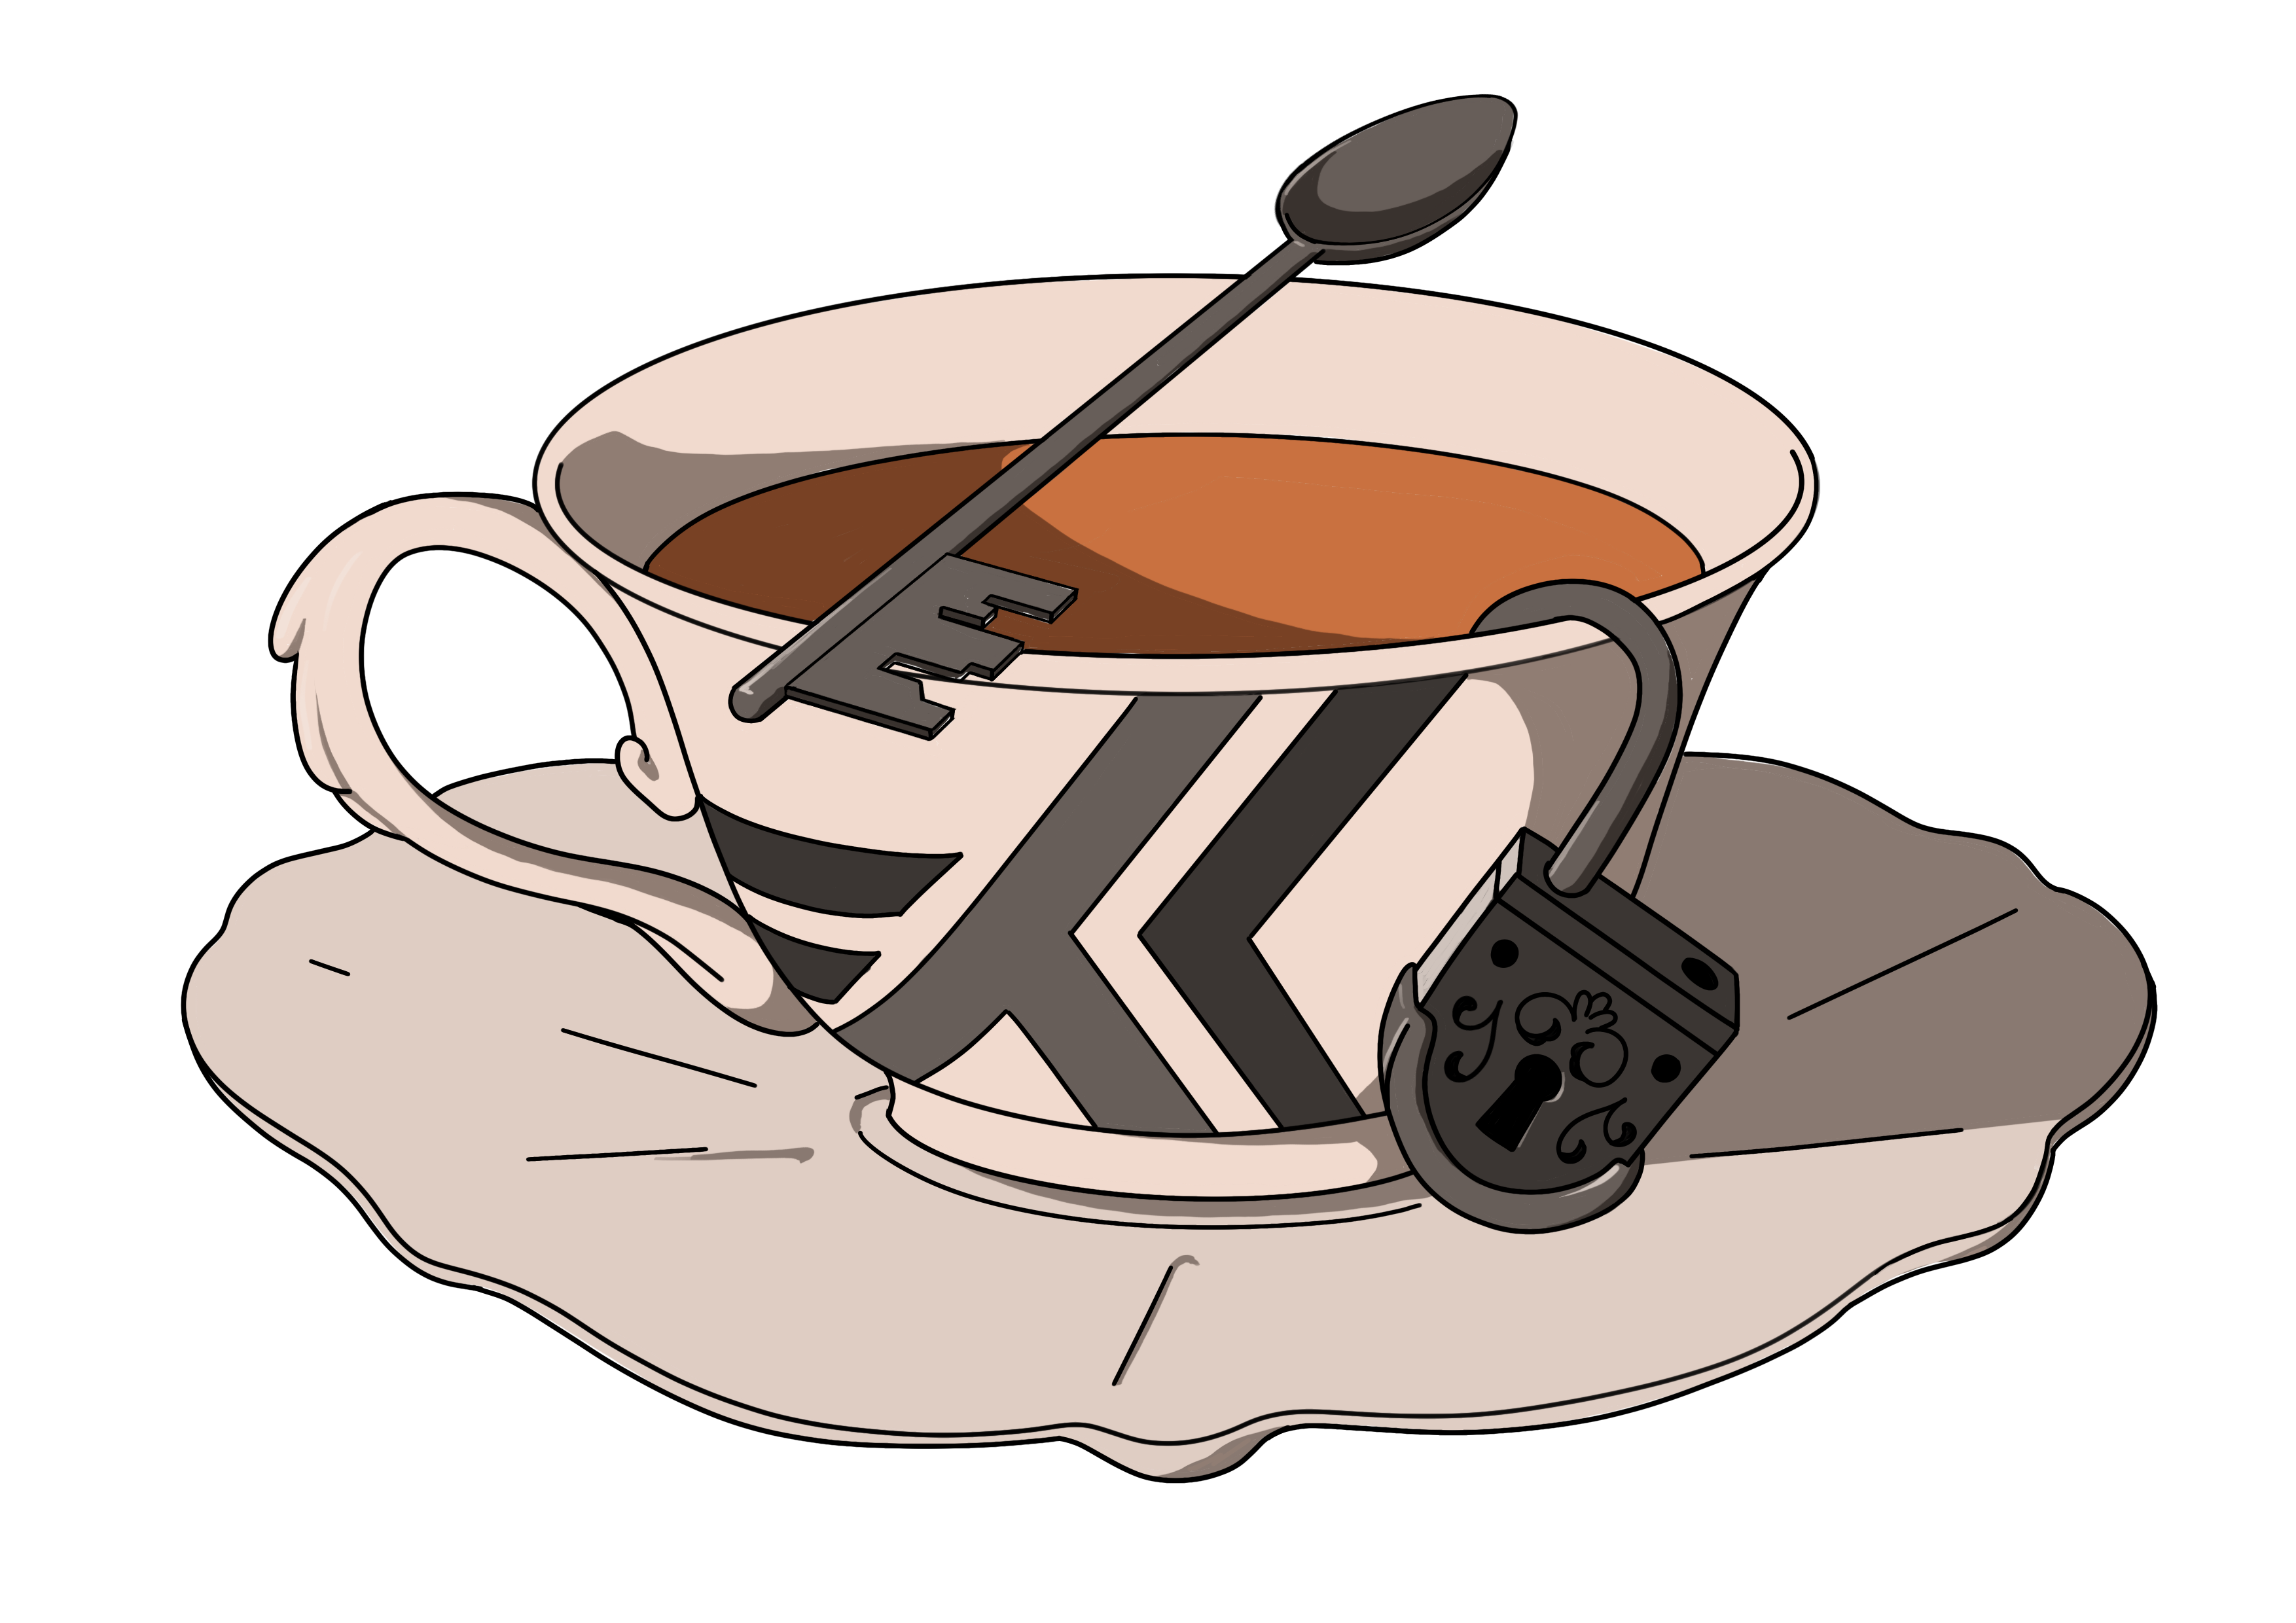
\includegraphics[scale=0.3]{graphics/HasTee_transparent.png}
\end{figure}

\vfill

\begin{center}
\textit{\mydepartment}\\
\textsc{\chalIgu}\\
Gothenburg, Sweden, \currentyear \\
\end{center}

%================================================================%
%                       Printing page                            %
%================================================================%
\newpage
\thispagestyle{empty}

\vspace{2cm} \noindent \textbf
\mytitle\\
\ifx\mysubtitle\undefined
\else
  \textit{\small\mysubtitle}
  \\
\fi

\noindent
\textsc{\authorname}\\

\vskip 0.5cm\noindent
\copyright \space \authorname,~\currentyear  \\
\noindent
except where otherwise stated. \\
All rights reserved. \vspace{1cm}


\vfill

\noindent \identifierNoText

\noindent 
\mydepartment\\
Division of \division\\
\ifx\researchgroup\undefined\else\researchgroup\\\fi
\chalIgu\\
SE-412 96 Göteborg,\\
Sweden\\
Phone: +46(0)31 772 1000

\vskip 1.5cm

Cover:\\
 Illustration by Andrea Svensson, \copyright \space Andrea Svensson
\\

\noindent
Printed by Chalmers Digitaltryck,\\
Gothenburg, Sweden \currentyear.


\setcounter{page}{1}
%The dedication.
\thispagestyle{plain}
\include{TexFiles/dedication}

%Abstract. Word length regulated by Chalmers/GU layouting guidelines.
\thispagestyle{empty} % To avoid page numbers in blank pages
\cleardoublepage \addcontentsline{toc}{chapter}{Abstract}
\thispagestyle{plain}
\begin{raggedright}
\noindent 
{\large\textbf{\mytitle}}\\
\ifx\mysubtitle\undefined\else\textit{\small\mysubtitle}\fi
\end{raggedright}

\vskip 1mm
\noindent
{\sc\authorname}
\vskip 1mm
\noindent
\textit{\mydepartment}\\
\textit{\chalIgu}

\vskip 8mm

\section*{Abstract}

\noindent

Without domain-specific language abstractions, developing software for niche domains can be a tedious, error-prone activity.
Notably, when the target platform of your application is a specific piece of hardware, the toolchain for that hardware
very often expects a developer to write low-level C code. C, for all the good it does, does not supply high-level abstractions,
much less domain-specific ones.

In this thesis I present my research on using Haskell to develop domain-specific languages for two specific domains, whose
intended target platform is not traditionally targeted by Haskell developers. The first application domain is real-time applications
for the Internet of Things, where the target platform is a microcontroller. The second application domain is
Confidential Computing, where the target platform is a conventional PC with support for hardware-enforced trusted execution
environments.

\vspace{10 mm}
\noindent{\textbf{Keywords}}

\vspace{3 mm}
\noindent{Haskell, Domain-specific languages, DSL, EDSL, Confidential Computing, Intel SGX, TEE}



%Publication list. NOT the actual papers.
\thispagestyle{empty} % To avoid page numbers in blank pages
\cleardoublepage \addcontentsline{toc}{chapter}{List of Publications}
\thispagestyle{plain}
%================================================================%
%                       Appended papers                          %
%================================================================%
\chapter*{List of Publications}
\label{chap:papers}

\section*{Appended publications}
This thesis is based on the following publications:

\newcommand{\pubitem}[3]{\item #1,
\newblock {\textit{#2}}\\
\newblock {\em #3}.
}

\begin{enumerate}[align=left,label={[\textbf{Paper \Roman*}]}]

    \pubitem{\textbf{R.~Krook}, J.~Hui, BJ.~Svensson, S.A.~Edwards, K.~Claessen}{Creating a Language for Writing Real-Time Applications for the Internet of Things}{20th ACM-IEEE International Conference on Formal Methods and Models for System Design (MEMOCODE) (October 2022), 1-20}
    \pubitem{A.~Sarkar, \textbf{R.~Krook},K.~Claessen,A.~Russo}{HasTEE: Confidential Computing on Trusted Execution Environments with Haskell}{In submission}

\end{enumerate}


% You might not need the following, remove it if so

\newpage
%================================================================%
%                        Other papers                            %
%================================================================%
\section*{Other publications}
The following publications were published during my PhD studies, or are currently in submission/under revision.
However, they are not appended to this thesis, due to contents overlapping that of appended publications or contents not related to the thesis.

\begin{enumerate}[align=left,label={[\textbf{\alph*}]}]
    \pubitem{N.~Valliappan, \textbf{R.~Krook}, A.~Russo, K.~Claessen}{Towards Secure IoT programming in Haskell}{Proceedings of the 13th ACM ISGPLAN International Symposium on Haskell (September 2020), 136-150}
    \pubitem{A.~Sarkar, \textbf{R.~Krook}, BJ.~Svensson, M.~Sheeran}{Higher-order Concurrency for Microcontrollers}{Proceedings of the 18th ACM SIGPLAN International Conference on Managed Programming Lanuages and Runtimes (September 2021), 26-35}

\end{enumerate}



%Acknowledgement
\thispagestyle{empty} % To avoid page numbers in blank pages
\cleardoublepage \addcontentsline{toc}{chapter}{Acknowledgement}
\thispagestyle{plain}
\chapter*{Acknowledgment}
\vspace{5 mm}

many thank

% I would like to thank my supervisor, Koen Claessen, for being a good friend and mentor. We have many interesting discussions
% together, of which only a fraction are about work!

% Aside from having a great supervisor, I am blessed with two excellent co-supervisors. In addition to saying that
% they are both great friends, I wish to thank John Hughes, for asking me the right
% questions and making me think, and Bo Joel Svensson, for his never ending support and trying to teach me to be a hacker, just like
% himself.

% There are too many friends, colleagues, and collaborators that deservers acknowledgements for a section as short as this one.
% I do, however, wish to single out Abhiroop Sarkar, for being a good friend and terrific office-mate.

% I wish to thank Troels Henriksen for agreeing to be my discussion leader, and for giving me feedback while I was
% writing on this thesis.

% Lastly, I wish to thank my family for their support, encouragement, and understanding. My greatest appreciation goes to my
% girls, Therese and Astrid, for helping me remember that there is a wonderful life to live outside of work.

% This work was funded by the Swedish Foundation for Strategic Research (SSF) under the project Octopi (Ref. RIT17-0023)

%================================================================%
% Table of contents, list of figures and tables
%================================================================%
\thispagestyle{empty} % To avoid page numbers in blank pages
\cleardoublepage
\thispagestyle{plain}
\tableofcontents 
\newpage

%If needed, lists of figures and tables
%\listoffigures
%\listoftables
 
\thispagestyle{empty} % To avoid page numbers in blank pages
\cleardoublepage

\mainmatter

%================================================================%
% Chapters
%================================================================%
\thispagestyle{empty} % To avoid page numbers in blank pages
\cleardoublepage 
\part{Summary}
\label{part:summary}
\newpage
\thispagestyle{empty} % To avoid page numbers in blank pages
\cleardoublepage 
\chapter{Introduction}
\label{chap:introduction}

\begin{figure}[h]
    \centering
    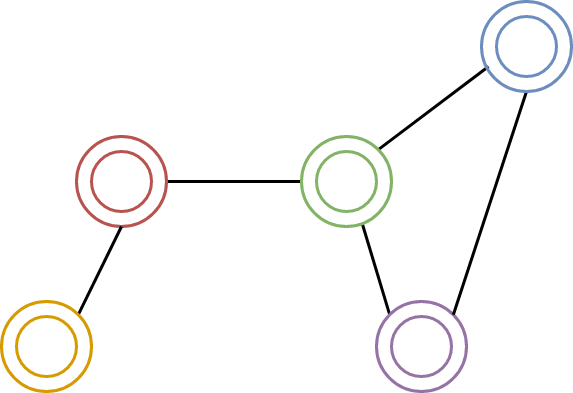
\includegraphics[scale=0.2]{graphics/mesh.png}
\end{figure}

Consider an application that is distributed over a network, e.g. as a set of \textit{Internet of Things}-devices (IoT). The
connection between devices forms a mesh network, and for the devices to be able to cooperate and implement the application they
need to agree on facts such as what the current time is, what other devices are part of the network, and more. In many cases
IoT devices take one of two roles. Either a device will perform period tasks such as reading a sensor and then transmitting
the value across the network to other devices, or a device will be idle until a value arrives from another device, at which point
the device needs to \textit{react} to that value.

The application described above has many moving parts that are non-trivial. The scarcity of hardware resources on many IoT
devices means that devices are often forced to rely on a battery for power. To ensure the continued availability of devices,
they need to carefully manage their power consumption such that the battery life is extended as far as possible. In addition to 
his, temporal properties need to be carefully stated and implemented. It could be crucial that a future action is
performed at a very precise moment in time. For devices to form a mesh network
and cooperate, the devices need to manage cryptographic keys. These keys are used to decide if a device is part of the network
or not and to ensure that a message in transit from one device to another is encrypted, such that the integrity of the network
is not violated.

The above requirements are very pervasive during the development of such an application and must be considered at every stage of
development. Devices such as these are usually programmed using low-level languages and toolchains such as C/C++. All the
requirements of the application above will require a lot of boilerplate code. Many things need to
happen to ensure that the requirements are met but don't relate to the application logic.

High-level languages offer different language abstractions that can more easily express the desired behavior of an application.
In addition, a language could offer domain-specific abstractions that ease application development for a specific domain.
As an example, aside from being a general-purpose language, Haskell's support for custom algebraic datatypes and pattern-matching
make Haskell excel at implementing programs that need to manipulate trees, such as compilers and interpreters. Erlang's support
for spawning concurrent processes that can communicate between endpoints in a network makes Erlang a good choice for implementing
applications that need to be distributed and scalable.

We ask ourselves a question; can we not leverage high-level languages with domain-specific abstractions to ease the
development of applications such as the one described at the top of this section? If the developer can be freed from the burden
of having to maintain boilerplate code, the developer can focus their energy on what the application is supposed to do, rather than
details of how it does it.

The topic of this thesis is to investigate whether it is feasible to develop a high-level language such as this. To
answer this, we develop DSLs that explore what domain-specific abstractions may be useful. The languages are
implemented as \textit{embedded} domain-specific languages (DSL) in the functional language Haskell. Embedding a DSL in a host
language drastically reduces the initial cost of language development, and enables experimentation to commence much quicker. An
embedded language can be implemented as an embedded compiler that generates code to be executed later, or as an embedded
interpreter that runs the program during host language execution time.

While we don't yet have a full story and a definitive answer, the work in this thesis brings us closer.
The thesis presents two DSLs, Scoria and HasTEE. Scoria investigates domain-specific
abstractions that help a developer specify the temporal behavior of their program. Additionally, the runtime system of Scoria can
recognize that a long period of inactivity is coming, and can choose to put the device it is running on in a low-power mode,
to conserve energy. While we have not evaluated how much power can be conserved yet, we believe it will be easy to evaluate
in the future. Scoria is intended to run on microcontrollers with scarce resources. Given the extensive runtime demands
of Haskell, it becomes infeasible to employ Haskell as the execution vehicle. Consequently, to address this limitation, Scoria
is implemented as an embedded compiler that generates C code. The C code is compiled at a later stage and executed on the device.

HasTEE develops domain-specific abstractions that ease the development of software with security requirements. Specifically,
HasTEE enables a developer to use the type system of Haskell to identify the parts of an application that are to be executed in a
trusted execution environment (TEE). The type system encodes a variant of information-flow control (IFC), but where traditional
IFC threat models require a developer to trust an underlying operating system, HasTEE does not require trust in an operating system.
A HasTEE application is automatically partitioned into two programs, an untrusted program and a trusted program, with the trusted
program being executed in a hardware-enforced TEE. The developer does not need to care about how confidentiality
is achieved when developing the application. HasTEE is intended to run on machines with more resources than that of the target
platform of Scoria, and as such is implemented as an embedded interpreter, where HasTEE uses the Haskell runtime as its execution
vehicle.

The results of this thesis indicate that there is space for a high-level language with domain-specific abstractions
that will ease application development in this domain, and there are many interesting lines of future work that could be pursued.
First, we wish to draw some synergy between Scoria and HasTEE, and enable a developer to write Scoria programs that use TEEs on
microcontrollers, e.g. Arm TrustZone on Cortex-M processors. Second, we wish to investigate if we can extend Scoria with
functionality to describe complete networks of devices and generate code for each of them. We wish to use the type system of
Haskell to identify unique devices and partition an application based on that.

The remainder of this thesis is structured as follows: first, the domains of the two DSLs presented in this thesis are
described in terms of an example application. The sections describe nuances related to application development of said domain,
and describe what domain-specific features might ease development. After that, a background section presents core topics that
are relevant to this thesis. Finally, the two papers follow.

% \begin{itemize}
%     \item The network is the computer - John Gage
%     \item Start from a high view, describing a distributed application with temporal behavior and
%     confidentiality requirements. From there, zone in on the difficulties with developing
%     these applications. (Low-level languages, power requirements, timing requirements, confidentiality requirements)
%     The impact is very pervasive
%     \item Low-level toolchains lead to a lot of code, which is more likely to be erroneous. Huge amount of
%     boilerplace code obfuscates application logic. Wish to use a high-level language to describe what the
%     application should do, without necessarily specifying how.
%     \item My plan - a high-level language for this
%     \item Embedded language development, quick prototyping, reuse components, high-level! Embedded compiler vs embedded interpreter.
%     \item Selling-point of HasTEE - partitioning and non-obfuscated application logic in the confidential component
%     \item Selling-point of Scoria - Time is native, sparse model, good for power requirements, High-level
%     \item Remaining work: Distributed Scoria, tierless programming, Arm TrustZone for confidential Scoria
% \end{itemize}

\section{Programs with Temporal Behaviors}

Consider a simple program
that flashes an LED at a fixed frequency. This program is the "Hello world!" of microcontroller programming, and is often distributed
as an example application with operating systems for microcontrollers. It illustrates how to perform
periodic tasks that do IO. The desired output should vary over time as illustrated in figure \ref{graphics:correct-frequency}.

\begin{figure}
    \centering
    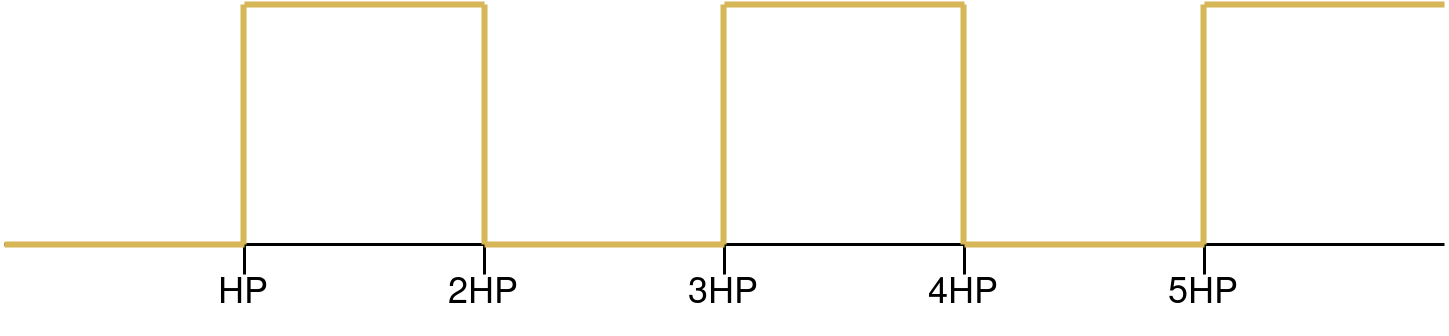
\includegraphics[scale=0.2]{graphics/correct-frequency.png}
    \caption{The yellow line denote the LED state and its desired temporal behavior. The desired behavior
    is that it is turned on and off with a stable frequency, with each change in state occuring at the
    half-period points, denoted \code{HP} in the diagram.}
    \label{graphics:correct-frequency}
\end{figure}

A pseudo-code variant of the program, as it is often illustrated, is shown below.

\begin{verbatim}
    void main() {
        while(1) {
            toggle_led(the_led);
            sleep(half_period);
        }
    }
\end{verbatim}

An equivalent version of the same program could use alarms and callbacks to specify what should happen at what time. Such
a version of the program appears below.
\begin{verbatim}
    void toggle() {
        toggle_led(the_led);
        set_alarm(half_period, &toggle);
    }

    void main() {
        configure_timer();
        set_alarm(half_period, &toggle);
    }
\end{verbatim}

The main function above configures some timer and sets an alarm that, when the alarm goes off, will trigger an invocation of
the \code{toggle} function. The \code{toggle} function flips the current value of the LED and then sets a new alarm.
While the code is very simple and seems to implement the desired semantics, it is buggy! The frequency will not be
the one we want. When the alarm goes off and the function is invoked, the function performs some operations before the next
alarm is set. If we call the time it takes to perform the operations $\delta_{op}$ and the half period $hp$, the times the
alarm goes off are $$0, \delta_{op} + hp, 2(\delta_{op} + hp), 3(\delta_{op} + hp), 4(\delta_{op} + hp), ...$$

This sequence illustrates that, as time progresses, the frequency drifts further and further away from the target. See
figure \ref{graphics:drift}.

\begin{figure}
    \centering
    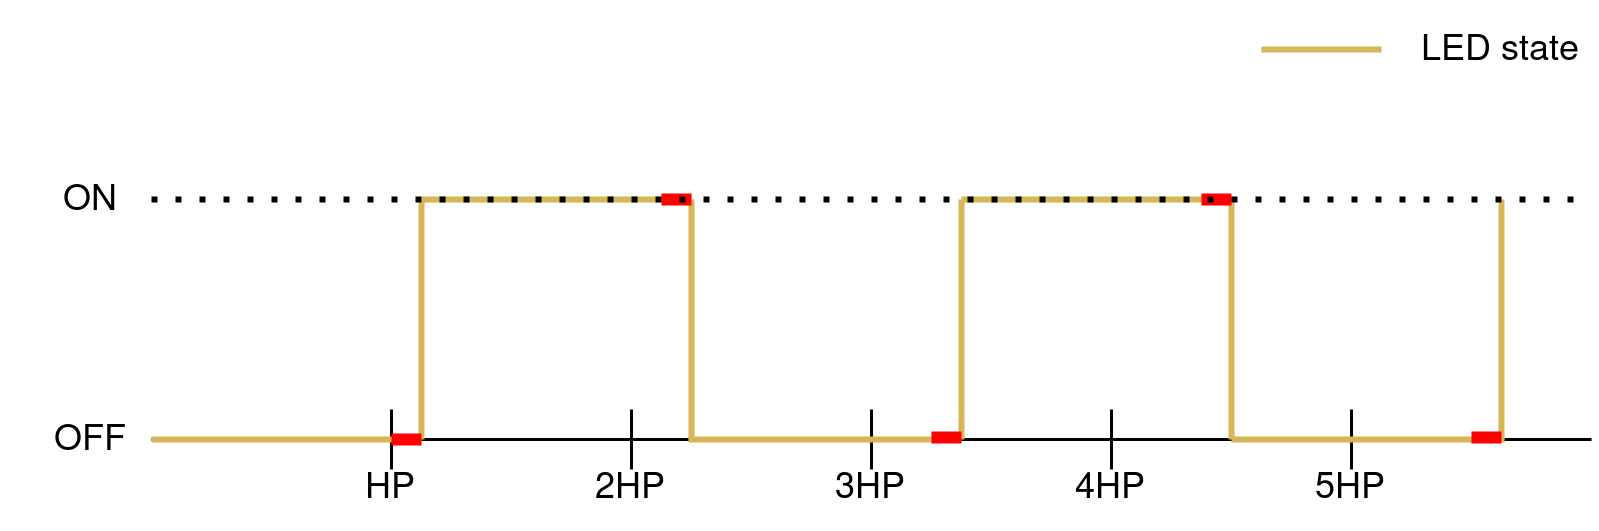
\includegraphics[scale=0.2]{graphics/drift.png}
    \caption{The diagram illustrates where the half-period points are, and where the change in LED state actually occurs.
    The red segments illustrate the time $\delta_{op}$. The additions of $\delta_{op}$ lead to the frequency of the change in
    LED state drifting further and further away from the half-period points.}
    \label{graphics:drift}
\end{figure}

Let us try to fix our program to allow for the time it takes to perform the operations.
As soon as \code{toggle} is invoked, we query the system for the current time. The next time we set
the alarm we configure the alarm to go off relative to the previously sampled time.

\begin{verbatim}
    time current;

    void toggle() {
        current = current_time();
        toggle_led(the_led);
        set_alarm_relative_to(current, half_period, &toggle);
    }

    void main() {
        configure_timer();
        current = current_time();
        set_alarm_relative_to(current, half_period, &toggle);
    }
\end{verbatim}

Even with the alarm set relative to when the process last woke up, the frequency suffers from drift. An oscilloscope
will report that the drift is smaller than before, but still present. This remaining source of drift is a bit
trickier to account for.

When the actual hardware clock reaches the point where an alarm should be raised, it takes some time for the
operating system to locate the \code{toggle} function and invoke it. To account for this delay, we can choose to
set alarms not relative to when \code{toggle} was last invoked, but rather relative to when \code{toggle}
\textit{was supposed} to have been invoked. We do this by implementing a logical clock that is incremented to reflect
what the time of the system should be.

\begin{verbatim}
    time current;

    void toggle() {
        current = current + half_period;
        toggle_led(the_led);
        set_alarm_absolute(current + half_period, &toggle);
    }

    void main() {
        configure_timer();
        current = 0;
        set_alarm_absolute(current + half_period, &toggle);
    }
\end{verbatim}

The program now maintains a global variable that tracks the current time. An absolute alarm is set that will go off at
time \code{current + half\_period}, regardless of what time it is when the alarm is set. The next time \code{toggle}
is invoked, it is assumed that time has progressed to \code{current + half\_period}, and the logical time is updated
to reflect this. If the system time is queried at this point, it will show that the current time is 
\code{current + half\_period +} $\delta_{lookup}$, where $\delta_{lookup}$ is the amount of time it takes for the
\code{toggle} function to be found and invoked.

Executing this program will flash the LED with the correct frequency. Since the delay for the system to look up and
invoke the callback ($\delta_{lookup}$) is still there, there is a small phase error (the size of which is equal to
$\delta_{lookup}$), but the frequency is still stable and correct. The LED state is illustrated in figure \ref{graphics:phase-error}

\begin{figure}
    \centering
    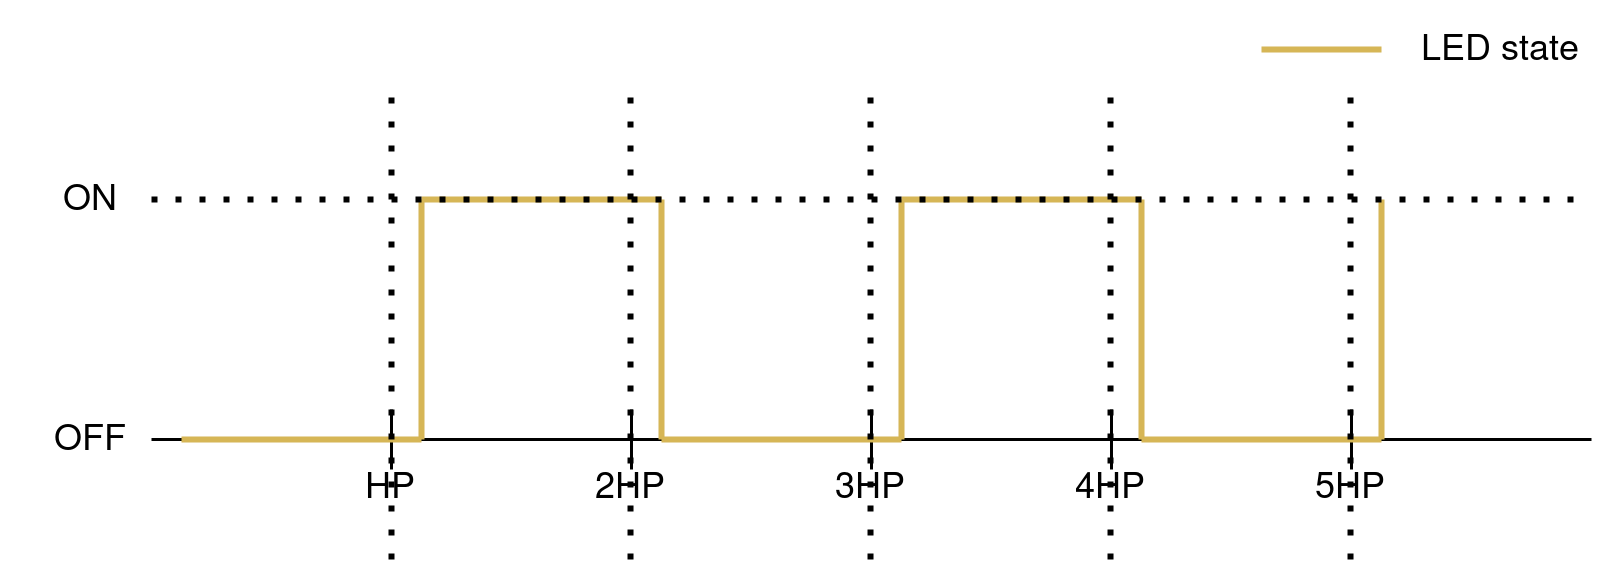
\includegraphics[scale=0.2]{graphics/phase-error.png}
    \caption{The diagram illustrates the frequency of the change in LED state in the final version of the program.
    There is a small phase error, indicated by the dotted lines, but otherwise the frequency is the expected one.
    The dotted lines denote the actual half-period points, and the distance from the points where the LED state
    changes to the half-period points remains constant. The distance is of duration $\delta_{lookup}$.}
    \label{graphics:phase-error}
\end{figure}

While the initial program seemed intuitively reasonable, it was actually erroneous. The final version is
correct (up to the phase error), but is substantially more complicated. While the pseudo-code might look short and
simple, still, we now have a program that maintains a logical time and sets absolute deadlines, something that is easy
to get wrong.

The extra complication is a result of the primitive timing API in a language such as this. Querying the system for the current
time and setting alarms is a very coarse API. The fact that the system does not assist the developer with accounting for
systematic delays and the time it takes to perform computations makes the whole business of reasoning about deadlines much more difficult.

Domain-specific abstractions that would make writing this program simpler are
\begin{itemize}
    \item An abstraction that schedules an alarm to go off after a certain amount of time
%    \item specify very precise periods of rest (where a software 'pauses') -- we can synthesize this
    \item An abstraction that yields control while awaiting an alarm
\end{itemize}

A developer should be able to use these primitives without thinking about systematic delays as the ones discussed above.
The logical time should be maintained by the runtime system. A rewrite of the above program using functionality of this
kind yields

\begin{verbatim}
    void main() {
        alarm a = new_alarm();
        while(1) {
            toggle_led(the_led);
            set_ds_alarm(half_period, shared);
            wait(shared);
        }
    }
\end{verbatim}

The program looks very similar to the first version, with the exception of using an explicit alarm instead of an
invocation of a \code{sleep} function.

The first paper in this thesis describes work on this domain. A domain-specific language, which we call
Scoria \cite{DBLP:conf/memocode/KrookHSEC22}, is implemented as an \textit{embedded} language in Haskell. While Scoria
has primitives similar to the ones described above, the alarms are more expressive. Alarms take the form of mutable
variable, which always have a value. An update to a mutable variable can be scheduled for the future, while a process can
choose to block until a mutable variable receives an update. The conceptual alarm goes off when the update occurs, and with
this alarm comes a value (the new value of the variable).

\begin{verbatim}
    signal_generator :: Ref Output -> Time -> SSM ()
    signal_generator led hp = routine $ while True $ do
        after hp led (invert $ deref led)
        wait led
\end{verbatim}

In this program, the LED variable itself becomes the alarm. In a while loop, a future update is scheduled for the LED
variable after which the program blocks until the update occurs. In Scoria, by writing to a variable associated
with an LED, the value of the LED is immediately propagated to the physical LED.

\section{Programs with Confidentiality requirements}

A second non-trivial application domain is that of confidential computing. Confidential computing is the act of protecting
\textit{data in use}.
Data always exists in one of three states. It can exist as \textit{data in motion}, as \textit{data at rest}, or as
\textit{data in use}. Data in motion is data that is moving from one part of the system to another, e.g. via TCP, while data at rest
is data that is being stored in persistent memory. Both of these kinds of data can be protected via e.g. encryption.
Encryption is enough to guarantee confidentiality in these cases if you trust your encryption scheme.

Data in use, however, is a bit different. To perform any meaningful operations on data, it has to be loaded in from
persistent storage. Consider the pseudo-code below

\begin{verbatim}
    (int, int) process_data(int x, int y) {
        return (x+2, x*y);
    }

    void server(key) {
        req          = await_request();
        (ct1, ct2)   = load_data(req);
        (pt1, pt2)   = (decrypt(ct1, key), decrypt(ct2, key));
        (r1,r2)      = process_data(pt1, pt2);
        (nct1, nct2) = (encrypt(r1, key), encrypt(r2, key));
        store((nct1, nct2));
    }
\end{verbatim}

The code consists of two parts. One part is the \code{server} function, which deals with communication and parsing of
incoming requests. The second part is actual application logic, which is very simple in this example. \code{server}
receives a request that indicates which confidential data should be loaded from the data storage. The data is decrypted before
it is handed off to the \code{process\_data} procedure, after which the result is encrypted and written back to data storage.

One problem with this code is that the data is decrypted before it is operated on. The result of this is that it exists in
plaintext form in the RAM of the machine the code is running on, and an attacker running on the same machine, such as a
compromised OS, might leak this data. This is illustrated
in figure \ref{graphics:unsafe-data-in-use}.

\begin{figure}
    \centering
    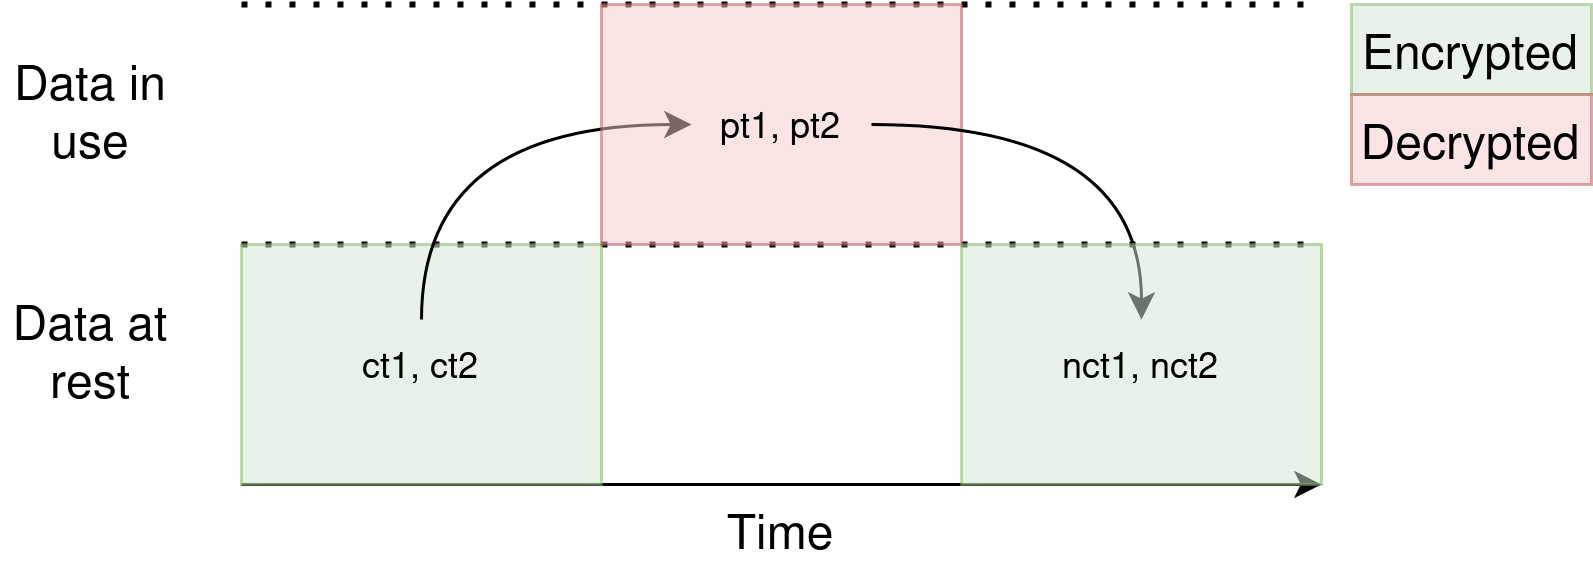
\includegraphics[scale=0.2]{graphics/unsafe-data-in-use.png}
    \caption{The diagram illustrates that while the data is at rest, it exists in encrypted form. When the data
    is operated on, it is loaded from the data storage and decrypted (as indicated by the red color), before the result is encrypted and
    written back to the data storage.}
    \label{graphics:unsafe-data-in-use}
\end{figure}

One technique for mitigating this is to apply homomorphic encryption\cite{DBLP:conf/stoc/Gentry09}. Homomorphic encryption is a form of encryption where
operations can be performed on the encrypted data without decrypting it, such that the decrypted result is the correct one.

\begin{verbatim}
    (int, int) process_data(int x, int y, Key key) {
        two   = encrypt(2, key);
        left  = homo_add(x, two, key);
        right = homo_mul(x,y, key);
        return (left, right);
    }

    server(key) {
        req          = await_request();
        (ct1, ct2)   = load_data(req);
        (r1,r2)      = process_data(ct1, ct2, key);
        store((r1,r2))
    }
\end{verbatim}

\begin{figure}
    \centering
    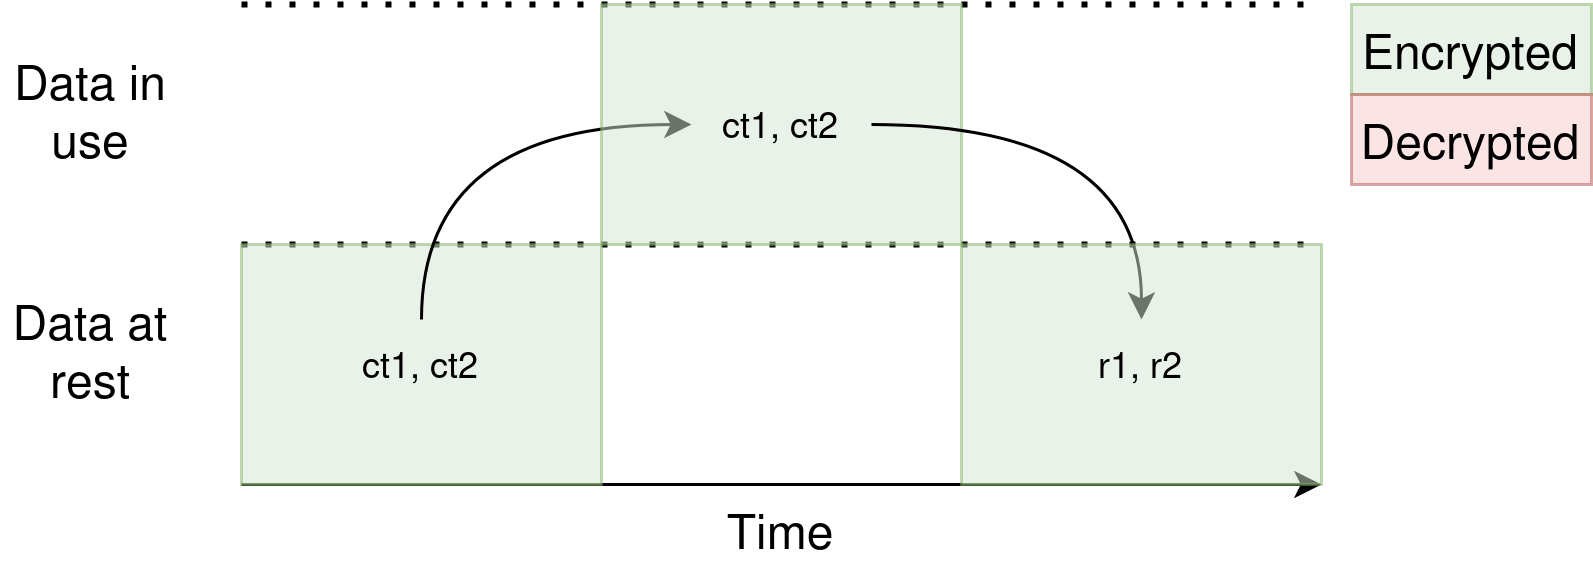
\includegraphics[scale=0.2]{graphics/safe-data-in-use.png}
    \caption{By applying homomorphic encryption, the data does not need to be decrypted before it is processed. The result
    of the computation is already encrypted, and is written back to the disk directly.}
    \label{graphics:safe-data-in-use}
\end{figure}

\textcolor{red}{FIXME: the key is still in RAM, need to say something about this}
In the above code, the data is never decrypted, as illustrated in figure \ref{graphics:safe-data-in-use}. Even if the OS is compromised, and the contents of the RAM leaked, the
data is not leaked in plaintext form. A downside of this approach is that the procedure that processes the data is now
much more complicated. It needs to apply special operations in place of ordinary ones. This obfuscates the code and
adds extra complexity. In the presence of a bug, it could also be harder to debug this code. While the example program
above still looks fairly simple, it does not scale very well.

Ideally, the program above would be described only in terms of the application logic. Encryption is an orthogonal part of
the application that just "needs to happen", and is not necessarily part of the application logic.

The problem is that the language does not have any abstractions that help describe what is confidential or not. It is all
implemented in software, where the developer has to explicitly handle encryption and decryption at correct points in the
code. A domain-specific abstraction for confidential computing would label the function \code{process\_data} as confidential,
and then the compiler would take over and actually ensure confidentiality.

\begin{verbatim}
    confidential (int, int) process_data(int x, int y) {
        return (x+2, x*y);
    }

    public server() {
        req          = await_request();
        (ct1, ct2)   = load_data(req);
        (r1,r2)      = execute_confidential(process_data(ct1, ct2));
        store((r1,r2))
    }
\end{verbatim}

\textcolor{red}{actually change the example to something that uses a secret stored in the enclave...}

This version of the program contains much less overhead in relation to application logic. The operation to be performed
on the data is described only in terms of application logic. There are no details of how confidentiality is ensured.

In the second paper of this thesis, we turn Haskell into a domain-specific language. The framework HasTEE is developed
which allows a developer to write a single Haskell application that uses two monads to describe which computations are
considered confidential, and which are not. This single Haskell application is then automatically partitioned into two
Haskell applications that communicate via remote procedure invocations, and then one of these applications will execute
inside a hardware enclave.

\textcolor{red}{Change the example above to be another one, and then implement that same example in HasTEE and show the reader that.}

\section{Background}

This section describe core topics that are relevant to this thesis. The first topic is \textit{Embedded Domain-specific Languages},
as the research presented in this thesis have been carried out by implementing embedded DSLs.
After this, a section about \textit{Synchronous Programming Languages} follow, as the DSL presented in paper one, Scoria, belongs
to the class of synchronous languages.
The last two topics relate to the DSL presented in paper two, HasTEE. They are \textit{Information-flow Control} and
\textit{Trusted Execution Environments}.

\subsection{Embedded Domain-specific Languages}

Implementing a programming language requires considerable engineering effort. At the very least, a parser and interpreter
has to be implemented. More than often there are many more phases involved, such as type checking, renaming, etc.

A lot of engineering effort can be spared by implementing a language as an embedded language. An embedded language is
implemented in another language, called the host language, as a library. By embedding a language in
a host language, many phases from the host compiler can be directly inherited by the new language, such as the parser,
type checker, code generator, etc.

Languages can be embedded in either a \textit{shallow} or \textit{deep} fashion.
While a shallow embedding will yield a result in a semantic domain, a deep embedding does not necessarily have to
do that. A deep embedding constructs syntax rather than evaluate semantics. This syntax can be interpreted at a later
stage to yield the semantics of a program. A deep embedding may also produce a value of another syntactic domain, by
\textit{generating code}. In such a scenario, we have two distinct execution times, the host language execution time, and the execution time of the generated
code, the embedded language. The host language becomes a very powerful meta-language for meta-programming in
the embedded language. This is a result of the two execution times -- the execution time of the host language and the
execution time of the embedded language. During host language execution time, programs in the embedded language can be
combined, manipulated, and optimized to produce other programs.

To illustrate this point we use an example from the Scoria language presented in this thesis.

\begin{verbatim}
    wait :: [Ref] -> SSM ()
    fork :: [SSM ()]
    procedure -- synthesize procedure
\end{verbatim}

The \code{wait} procedure takes a list of references as input, and blocks until \textit{either} of them has received an update.
\code{fork} spawns any number of concurrent child processes, and blocks until \textit{all} of them have terminated.
\code{procedure} takes a Haskell function body and turns the function into a procedure in the embedded language.

Something missing from Scoria, but that we can implement with the help of the host language, is a variant of the
\code{wait} procedure that blocks until \textit{all} references have received updates.

\begin{verbatim}
    waitSingle :: Ref -> SSM ()
    waitSingle ref = procedure $ do
        wait [ref]
    
    waitAll :: [Ref] -> SSM ()
    waitAll refs = fork $ map waitSingle refs
\end{verbatim}

\code{waitSingle} creates an embedded Scoria procedure which, during Scoria execution time, waits for a
single reference to receive an update. \code{waitAll} is a Haskell function which, during Haskell execution time, takes a list of
references and produces a \code{fork} statement that, during Scoria execution time, produces child processes that each
invoke \code{waitSingle} with one of the references. Since \code{fork} does not terminate until all child processes
terminate, \code{waitAll} will not terminate until all references received updates. The code exploits the fact that
\code{waitAll} is executed during Haskell execution time, and expands into code that is executed during Scoria execution time.

A code-generating EDSL can exploit the two execution times to perform partial evaluation\cite{DBLP:conf/haskell/ValliappanRL21},
by specializing the embedded program during the host language execution time. A compiler optimizes a program by applying
rewrite rules, turning a value of a syntactic domain into another value of the same syntactic domain.
By embedding a language inside a host language, the host language can transform program fragments of the embedded language
into values of a semantic domain that the host language can evaluate. The result of this evaluation can then be reified to
yield a new value in the syntactic domain again.

While these are some arguments in favor of EDSLs over DSLs, there are also arguments against EDSLs. Three of the more prevalent
arguments against EDSLs are

\begin{itemize}
    \item The syntax of the embedded language is influence by the choice of host language. A dedicated DSL will have its own
    parser that supports domain-specific syntax.
    \item The choice of host language can have an impact on developer efficiency. If a language is embedded in e.g. Haskell, a
    Haskell developer is better situated to exploit Haskell features to write clever programs.
    \item As an embedded program is written in a host language, error messages from the host language are inherited. These may
    be more complicated than necessary, and can reflect implementation details that don't concern the application developer.
\end{itemize}

\textcolor{red}{Perhaps reiterate that for language prototyping, we can be very efficient with an EDSL. We can then
develop an actual DSL after we are done experimenting, and have a better idea of what we want our language to look like.}

% that the syntax of the embedded language becomes influenced by the host language. A dedicated DSL will employ its own parser,
% yielding potential domain-specific syntax that simplifies program development. Another argument is that the choice of host language
% might impair programmer efficiency. If an EDSL is embedded in e.g. Haskell, a Haskell developer might be much more efficient
% than a C developer, as the Haskell developer knows how to properly take advantage of the host language features.

\subsection{Synchronous Programming Languages}

A \textit{reactive} program is one that rects to events. Events are delivered via streams, and are either present or absent.
Hardware designers have taken this paradigm to heart and have engaged in \textit{dataflow} programming for many decades.
A dataflow program structures a program as a collection of nodes, connected via directed edges, through which data (events) are
transmitted. An event can either be present or absent, and when all incoming edges of a node have a value, the node will
immediately compute values for its outgoing edges, conceptually instantaneously. In this context of hardware, edges always
carry a value (a zero or a one), and upon every cloc of the processor, the whole system is updated.

Drawing inspiration from this, french researchers in the 1980s did seminal work on \textit{synchronous} languages in the
form of the languages Lustre \cite{DBLP:conf/popl/CaspiPHP87}, Esterel \cite{DBLP:journals/scp/BerryG92},
and Signal \cite{DBLP:journals/scp/BenvenisteGJ91}. Lustre and Signal are dataflow languages, while Esterel
is an imperative language.

The two main concepts in Lustre are those of \textit{streams} and \textit{nodes}. A stream is an infinite sequence of values,
where a value need not be present at every instant. Consider the stream \code{X} that counts up at every instant, and
the stream \code{EVEN} that filters out the even numbers.

\begin{verbatim}
    instant 1,2,3,4,5,6,7,8,9,10,11,12,...

    X    =    [1,2,3,4,5,6,7,8,9,10,...
    EVEN =    [  2,  4,  6,  8,  10,...
\end{verbatim}

Whereas \code{X} is present at every instant, \code{EVEN} is only present at every other instant. New streams can be computed
from existing streams.

\begin{verbatim}
    X     = [1,2,3,4,5,...
    Y     = [6,2,3,4,9,...
    X + Y = [7,4,6,8,14,...
\end{verbatim}

The expression \code{X + Y} is only valid if \code{X} and \code{Y} are defined in the same instants. The expression
\code{X + Y} has no meaning if either \code{X} or \code{Y} doesn't have a value, and the program is rejected by the Lustre
compiler. It is common to refer to a stream as having a \textit{clock} that ticks at those instants where a value is
present. In the example with the streams \code{X} and \code{EVEN}, the clock of \code{X} ticks at a certain rate and
the clock of \code{EVEN} ticks at half the rate of \code{X}.

As streams such as \code{X + Y} depend on other streams, \code{X + Y} \textit{reacts} when \code{X} and \code{Y} are
present. Reactions such as these are conceptually instantaneous, giving rise to the term \textit{synchronous} languages,
as outputs are computed synchronized with when their inputs appear.

Reusable nodes can be declared. A node takes a number of input streams as arguments and produce output streams. When events
arrive on the input streams, the node immediately \textit{reacts} and compute values for its output streams. The node below
implements a counter whose output stream is a growing sequence, that can be reset when the \code{reset} stream is \code{true}.

\begin{verbatim}
    node COUNTER(val_init, val_incr: int; reset: bool)
        returns (n: int);
    let
      n = val_init -> if reset
                      then val_init
                      else pre(n) + val_incr;
    tel.
\end{verbatim}

Esterel takes a different view at synchronicity. Instead of nodes in a dataflow graph reacting to input events, Esterel
declares nested threads that may react to broadcasted signals. Threads may suspend while waiting for a signal, and when
the signal is broadcasted in an instant, the thread reacts instantaneously. The signal does not persist until the next
instant. Esteral is an imperative language with common control-flow statements, such as loops and conditionals.

\textcolor{red}{write more on Esterel, of course}

Common to all these synchronous languages is that despite being able to create clocks and use them to specify
temporal behavior, the programs are still ultimately governed by a global clock. Upon every tick of this clock, the program
reacts, as shown in figure \ref{graphics:global-clock}. Furthermore, while being suitable for specifying temporal
properties, it is not actually possible to specify temporal properties directly! A program may react to a signal or event,
but that event need not be synchronized with time. It is possible to, in one instant, specify behavior in relation to other
instants, but not in relation to time. These languages does not have an abstraction that let's the developer e.g. say
\textit{wait for two seconds}, but rather have abstractions that express \textit{wait for an event}. It is then up to the
runtime system to provide a source of events that can be used to define a two second delay.

Stephen A. Edwards and John Hui \cite{DBLP:conf/fdl/EdwardsH20} recognized that broadcasting an event at every tick of a global clock can be
wasteful. In some application domains, such that that of \textit{Internet of Things}, many tasks are periodic. There are
long periods of time where no action should be taken, and during these periods, no event should be broadcasted. This lets
the device the program executes on conserver power. This observation, together with a desire to be able to specify concrete,
temporal behavior, lead to the \textit{Sparse Synchronous Model} (SSM).

In SSM, not all instants are broadcasted to a program, as shown in \ref{graphics:sparse-clock}. \textcolor{red}{The figure mentions a step function. Either mention this in the text, or remake the figure} Temporal behavior such as
\textit{wait for two seconds} can be expressed natively. Time is a first-class citizen, and can be treated as any other value.
A SSM program is made up of threads, similar to Esterel. Threads may spawn other threads and communicate to them via signals.

\begin{verbatim}
foo(&a)
  wait a
  a = a * 2

bar(&a)
  wait a
  a = a + 4

main()
  var a = 0
  after (1 second) a 1
  fork bar(a), foo(a)
\end{verbatim}

In the above example, the variable \code{a} is used to transmit signals. The \code{fork} statement will spawn concurrent
child processes \code{bar} and \code{foo}. The processes block until \code{a} receives an update, which it does after one second,
as scheduled by the \code{main} procedure before the children were forked. To ensure determinism, processes are ordered. The
above program will first give \code{a} the value \code{1} when one second has passed, after which \code{bar} wakes up and
adds \code{4} to it. Then \code{foo} wakes up and multiplies \code{a} with two, yielding a final value of \code{10} for \code{a}.

Another more recent synchronous language is Lingua Franca (LF) \cite{DBLP:journals/tecs/LohstrohMBL21}. LF uses the abstraction
of reactors instead of threads or nodes. Actors are used to model concurrent processes in languages such as Erlang. Actors
communicate by sending messages to each other, but allows for nondeterminism by not ordering messages.
The reactors in LF assign an ordering to every message, yielding a deterministic program.
A LF program declares a static dataflow graph, whereas SSM defines a dynamic dataflow graph that grows and shrinks as the
program is running.

\begin{figure}
    \centering
    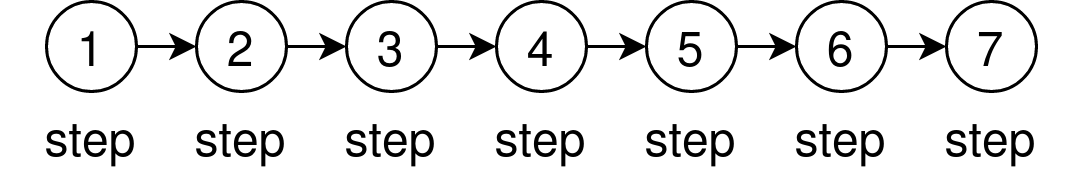
\includegraphics[scale=0.2]{graphics/clock-governed.png}
    \caption{Upon each tick of the global clock, the step function is invoked, and the whole program
    is evaluated for the instant denoted by the index of the tick.}
    \label{graphics:global-clock}
\end{figure}

\begin{figure}
    \centering
    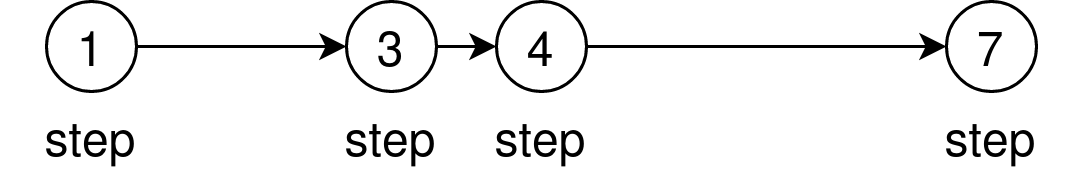
\includegraphics[scale=0.2]{graphics/sparse-clock.png}
    \caption{In contrast to the synchronous model, the sparse synchronous model allows the runtime system to
    detect that no computation should take place for some time. Not having to invoke the step function
    leaves the system open to perform other tasks, and if none exist, to sleep and conserve energy.}
    \label{graphics:sparse-clock}
\end{figure}

\subsection{Information-flow Control}

\todo{rephrase the first part, and slide into IFC in a better way.}
Information-flow control (IFC)\cite{DBLP:series/natosec/HedinS12} ensures that data propagates through a program in such a way that some security policy is
not violated. Values are labeled with a security level, which is then tracked when a value is used to make sure that the
value is not used inappropriately.
A value of one security level can e.g. not influence the result of a value with a lower security level. The property that no data is leaked
in this way is called noninterference.

As a simple example, we describe a language with two security levels, public and secret. We assume that anyone can inspect
a program's public output. The pseudo-code below denotes security levels explicitly in the type signature
of the procedure.

\begin{verbatim}
    public int f(secret int x, public int y) {
        y = x;
        return y;
    }
\end{verbatim}

The above program is ill-formed, as the secret input is assigned to the public output before it is returned. This is an
explicit leakage of information. Implicit leakages are also possible, as in the program below.

\begin{verbatim}
    public bool f(secret bool x, public bool y) {
        if(x) {
            return y;
        } else {
            return (not y);
        }
    }
\end{verbatim}

By inspecting the output we can infer what the secret input was, even though we never directly assign the secret input
to the public variable \code{y}. Note that in both cases, the program would be accepted if we labeled the output as secret.

IFC policies can be enforced statically, dynamically, or through a combination of both. A static policy is checked before
a program is allowed to execute, whereas a dynamic policy is checked at runtime. If the policy is violated, execution
is aborted and an error is raised.

If a value could \textit{never} be downgraded to a lower security level, however, then it would be difficult to write any meaningful program that uses
different security levels. A principled way to release secrets is to explicitly declassify values, giving them a lower
security level.

\begin{verbatim}
secret string stored_pass;

public bool check_password(public string password) {
    secret outcome = compare(stored_pass, password);
    return declassify(outcome);
}
\end{verbatim}

The result of comparing the stored password against the candidate password must be secret, as we had to use the secret stored
password to do the comparison. Before the resulting boolean can be released as a public outcome, we must
\code{declassify} it.

Regardless of whether you use static IFC, or dynamic IFC, or a hybrid variant of IFC, the threat model assumes that the
operating system and runtime system are trusted. In the presence of a compromised operating system, which we assume can
inspect any memory it desires, it does not matter what label a piece of data has. The operating system can inspect and
leak it.

\textcolor{red}{TODO write something more maybe}

\subsection{Trusted Execution Environments}

In an effort to protect data in use, every major hardware vendor is working on support for hardware-enforced trusted
execution environments (TEE). Intel is developing its Intel Software Guard Extensions (Intel SGX)\cite{intelsgx}, Arm is
developing Arm TrustZone\cite{armtz}, AMD is developing different variants such as AMD-SEV\cite{amdsev}, AMD-SME, and
AMD-SEV-SNP, to name just a few. A TEE allocates a contiguous region of memory that contains both secure code and data.
This region of memory is then protected by the hardware, where the protection mechanism varies between hardware vendors.
The purpose is that e.g. a compromised operating system can not read this memory.

Intel SGX refers to such protected memory regions as \textit{enclaves}, and protect them via encryption by the CPU. Code and
data is decrypted when it moves into CPU cache, and encrypted when it leaves the CPU cache. This constant encryption
and decryption add significant overhead. When untrusted code invokes a trusted method in an enclave, the time it takes
to just perform the function call is upwards of 35 times slower.

In contrast to Intel SGX, Arm TrustZone use hardware isolation to separate the memory accessible by untrusted software and
trusted software. No encryption is needed, as untrusted memory can not access trusted memory. \textcolor{red}{ask abi for performance}

The programming model for TEEs requires the developer to partition their application into two components. One component
executes inside the TEE, while the untrusted component executes outside. The untrusted components drive the execution, and may
perform remote procedure calls in the application inside the TEE, which in turn can call out of the enclave if it requires so.
If untrusted code tries to access trusted data, an error will be raised. This configuration is illustrated in
figure \ref{graphics:tee}.

\begin{figure}
    \centering
    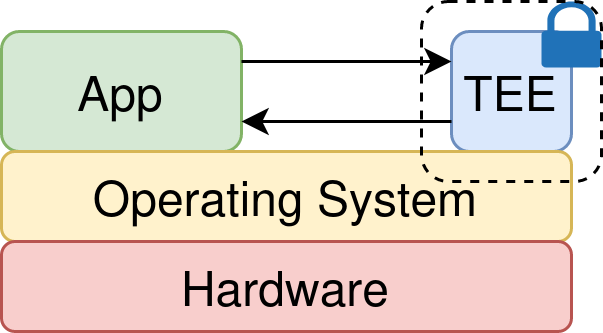
\includegraphics[scale=0.2]{graphics/tee.png}
    \caption{The diagram illustrates that an application using a hardware-enforced TEE to protect its secrets need to
    be partitioned into two parts. The part outside of the TEE can perform remote procedure calls in the application
    executing inside the TEE. Arrows indicate remote procedure invocations.}
    \label{graphics:tee}
\end{figure}

While this sounds simple enough, it is in practice quite complicated. Aside from technical complexity
concerning the maintenance of toolchains, actual application development is not trivial. Managing two projects and an
interface between them takes some effort. The TEE application is much more restricted in what it can do as some
operations are inherently leaky. As an example, applications intended to run on Intel SGX need to be compiled with a
restricted version of the C standard library, where many ordinary functions are missing. This makes it difficult to port
legacy applications to run on Intel SGX, as these applications were written with the assumption that they can access the
whole standard library. To ease the porting of legacy applications to Intel SGX, projects such as Gramine have emerged
(previously called Graphene \cite{DBLP:conf/usenix/TsaiPV17}). Gramine is a library OS that reintroduces the missing
functionality from the restricted standard library, enabling any Linux binary to run unmodified.

% \section{This Thesis}

% The research described in this thesis details my experimentation and exploration of the design and implementation of
% DSLs, where I feel that there are unexplored abstractions that warrant experimentation.

% In paper 1 I experiment with language design for a language that treats time as a first-class citizen. The programming model
% is implemented with support for IO, and the intention is that it should be easy to specify the temporal behavior of a program
% without needing to worry about the details of implementation.

% In paper 2 we turn Haskell itself into a DSL for writing applications that use secure enclaves. We implement a library that
% allows the developer to specify which computations should happen inside an enclave, and which should happen outside. We
% then recognize that such a scenario is equivalent to enforcing IFC policies, but in a system where the operating system
% does not have to be trusted.

% \section{Future work}

% My research has reached a point where there are many different paths forward. Below I will mention a few of them.

% \begin{itemize}
%     \item Is it possible to distribute Scoria? Currently, SSM executes locally on a single machine, but it would be interesting
%     to see how it could be distributed to execute across multiple devices in a network. Latencies in network communication
%     might lead to an event arriving after time has already progressed. Related work to this is e.g LF \cite{DBLP:journals/tecs/LohstrohMBL21} and PTIDES \cite{DBLP:conf/dsrt/DerlerLM08}.
%     \item Generalizing HasTEE such that more than one TEE can be programmed would allow
%     us to use a more general lattice of security label, rather than the binary system of labels we currently use (trusted/untrusted).
%     \item To further increase trust in a HasTEE application, it should be investigated whether the attestation functionality of
%     e.g Intel SGX can be used to prove the trustworthiness of the generated enclaves.
%     \item HasTEE applications do not make any assumptions on the underlying hardware TEE. We wish to investigate if we can port
%     HasTEE to other hardware platforms, such as Arm TrustZone.
%     \item We would like to explore whether there can be some synergy between Scoria and HasTEE. Some microcontrollers come with
%     the Arm Cortex-M processors, which have support for TrustZone. It would make for a very nice story if all of these things can come
%     together; distributed SSM with support for confidential computing.
% \end{itemize}



% My research so far have taken me to a place where there are many potential ways foward. My work on Scoria showed how we can
% extend a reactive system with support for IO, while remaining deterministic. My work on HasTEE illustrated that is it possible
% to perform confidential computing in native Haskell, with the use of a simple library.



%%%%%%%%%%%%%%%%%%%%%%%%%%%%%%%%%%%%%%%%%%%%%%%%%%%%%%%%%%%%%%%%%%%%%%%%%%%%%%%%%%%
%%%%%%%%%%%%%%%%%%%%%%%%%%%%%%%%%%%%%%%%%%%%%%%%%%%%%%%%%%%%%%%%%%%%%%%%%%%%%%%%%%%

% \chapter{Summary of Included Papers}
% \label{chap:summary}

% \section{Title of the First Paper}
% \sectionmark{First Paper} % This is in case the title is too long to fit properly in the headings of the following pages

% In this paper we present a method to do something.

% \subsubsection*{Problem}

% Description of what we are trying to solve.

% \vskip 1cm

% Lorem ipsum dolor sit amet, consectetur adipiscing elit, sed do eiusmod tempor incididunt ut labore et dolore magna aliqua. Vel facilisis volutpat est velit egestas dui. Enim ut sem viverra aliquet eget. Lorem sed risus ultricies tristique nulla aliquet. Ultricies mi eget mauris pharetra et ultrices neque. Gravida rutrum quisque non tellus orci ac auctor augue mauris. In fermentum et sollicitudin ac orci phasellus egestas tellus. Orci ac auctor augue mauris augue neque gravida. Facilisi morbi tempus iaculis urna id volutpat lacus laoreet non. Hac habitasse platea dictumst vestibulum. Egestas fringilla phasellus faucibus scelerisque eleifend donec pretium. Auctor elit sed vulputate mi sit amet mauris commodo quis. Vitae nunc sed velit dignissim sodales ut.



% \subsubsection*{Contribution}

% What does the paper do to try to solve the problem?

% \vskip 1cm

% Molestie a iaculis at erat. In vitae turpis massa sed elementum tempus. Tincidunt id aliquet risus feugiat in ante metus. Nunc sed blandit libero volutpat. Pharetra diam sit amet nisl. Eu facilisis sed odio morbi quis commodo odio. Porta lorem mollis aliquam ut porttitor. Metus vulputate eu scelerisque felis imperdiet. Volutpat sed cras ornare arcu dui vivamus arcu felis bibendum. Ultrices mi tempus imperdiet nulla. Tristique sollicitudin nibh sit amet commodo nulla facilisi nullam. Tortor vitae purus faucibus ornare suspendisse sed. Quisque id diam vel quam elementum pulvinar etiam non. Platea dictumst vestibulum rhoncus est pellentesque.


% \subsubsection*{Methodology}

% How is it implemented?

% \vskip 1cm

% Consequat nisl vel pretium lectus quam id. Phasellus egestas tellus rutrum tellus. Id neque aliquam vestibulum morbi blandit cursus risus at ultrices. Est ultricies integer quis auctor elit sed vulputate. Eu consequat ac felis donec et odio pellentesque diam volutpat. Urna id volutpat lacus laoreet non curabitur gravida arcu ac. Scelerisque purus semper eget duis at tellus. Porttitor leo a diam sollicitudin tempor id eu nisl nunc. Mauris nunc congue nisi vitae suscipit tellus mauris. Leo duis ut diam quam nulla porttitor massa id neque. In hendrerit gravida rutrum quisque non. Ornare lectus sit amet est.


% %%%%%%%%%%%%%%%%%%%%%%%%%%%%%%%%%%%%%%%%%%%%%%%%%%%%%%%%%%%%%%%%%%%%%%%%%%%%%%%%%%%
% \clearpage

% \section{Title of the second paper}

% In this paper we present a method to do something else.


% \subsubsection*{Problem}

% Description of what we are trying to solve.

% \vskip 1cm

% Lorem ipsum dolor sit amet, consectetur adipiscing elit, sed do eiusmod tempor incididunt ut labore et dolore magna aliqua. Vel facilisis volutpat est velit egestas dui. Enim ut sem viverra aliquet eget. Lorem sed risus ultricies tristique nulla aliquet. Ultricies mi eget mauris pharetra et ultrices neque. Gravida rutrum quisque non tellus orci ac auctor augue mauris. In fermentum et sollicitudin ac orci phasellus egestas tellus. Orci ac auctor augue mauris augue neque gravida. Facilisi morbi tempus iaculis urna id volutpat lacus laoreet non. Hac habitasse platea dictumst vestibulum. Egestas fringilla phasellus faucibus scelerisque eleifend donec pretium. Auctor elit sed vulputate mi sit amet mauris commodo quis. Vitae nunc sed velit dignissim sodales ut.



% \subsubsection*{Contribution}

% What does the paper do to try to solve the problem?

% \vskip 1cm

% Molestie a iaculis at erat. In vitae turpis massa sed elementum tempus. Tincidunt id aliquet risus feugiat in ante metus. Nunc sed blandit libero volutpat. Pharetra diam sit amet nisl. Eu facilisis sed odio morbi quis commodo odio. Porta lorem mollis aliquam ut porttitor. Metus vulputate eu scelerisque felis imperdiet. Volutpat sed cras ornare arcu dui vivamus arcu felis bibendum. Ultrices mi tempus imperdiet nulla. Tristique sollicitudin nibh sit amet commodo nulla facilisi nullam. Tortor vitae purus faucibus ornare suspendisse sed. Quisque id diam vel quam elementum pulvinar etiam non. Platea dictumst vestibulum rhoncus est pellentesque.


% \subsubsection*{Methodology}

% How is it implemented?

% \vskip 1cm

% Consequat nisl vel pretium lectus quam id. Phasellus egestas tellus rutrum tellus. Id neque aliquam vestibulum morbi blandit cursus risus at ultrices. Est ultricies integer quis auctor elit sed vulputate. Eu consequat ac felis donec et odio pellentesque diam volutpat. Urna id volutpat lacus laoreet non curabitur gravida arcu ac. Scelerisque purus semper eget duis at tellus. Porttitor leo a diam sollicitudin tempor id eu nisl nunc. Mauris nunc congue nisi vitae suscipit tellus mauris. Leo duis ut diam quam nulla porttitor massa id neque. In hendrerit gravida rutrum quisque non. Ornare lectus sit amet est.



% %%%%%%%%%%%%%%%%%%%%%%%%%%%%%%%%%%%%%%%%%%%%%%%%%%%%%%%%%%%%%%%%%%%%%%%%%%%%%%%%%%%
% %%%%%%%%%%%%%%%%%%%%%%%%%%%%%%%%%%%%%%%%%%%%%%%%%%%%%%%%%%%%%%%%%%%%%%%%%%%%%%%%%%%

% \chapter{Discussion and Future Work}
% \label{chap:discussion-future-work}

% What are your conclusions?

% What's next?


%%================================================================%
%% Bibliography
%%================================================================%
\newpage
\thispagestyle{empty} % To avoid page numbers in blank pages
\cleardoublepage\addcontentsline{toc}{chapter}{Bibliography}

% Choose citation styles depending on whether you want numeric/alphabetic in settings.tex
\printbibliography


%================================================================%
% Appended papers
%================================================================%
%The actual papers that are included in the thesis
% \newpage
% \thispagestyle{empty} % To avoid page numbers in blank pages
% \cleardoublepage 
% \part{Appended Papers}
% \newpage
% \thispagestyle{empty} % To avoid page numbers in blank pages
% \cleardoublepage 

% \include{TexFiles/appendedPapers}


%
%================================================================%
% Appendices
%================================================================%
%\cleardoublepage
%I place all appendices at the end of the thesis. Of course, you can also change this so that each appendix is directly following the paper it belongs to.
%\addcontentsline{toc}{chapter}{Appendix}
%\appendix
%\chapter{Appendix - Paper A}
%\input{papers/paperA/03_appendix}


\end{document}
